\chapter{Software for emotion detection}
\label{ch:software}

This chapter details the software developed to be an instanciation of the artifact produced as the outcome of this research, which is an approach for remotely detecting the changes in stress and boredom levels of a player during the interaction with a game. The software is developed in C++ and its overall structure is illustrated in Figure \ref{fig:tool-overall-structure}.

\begin{figure}[h]
    \centering
    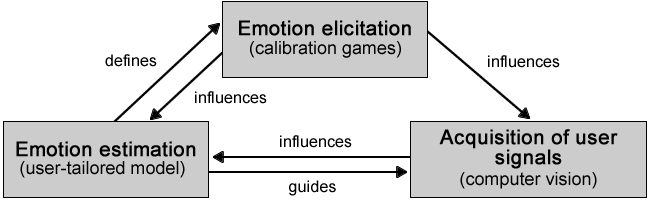
\includegraphics[width=0.8\textwidth]{figures/method-components-dependency.png}
    \caption{Overall structure of the software. Components highlighted in red are unfinished.}
    \label{fig:tool-overall-structure}
\end{figure}

The software contains six main components: face detector, signal estimator, face analyzer, emotion model manager, emotion estimator and finally report manager. The two components marked in read, the emotion model and the emotion estimator, are responsible for emotion estimation. Those components are unfinished and will be implemented in the future. The remaining of the components is finished and working. The following sections detail those components.

\section{Face detector}

The face detector component locates a human face in a frame of the of input video being analyzed. It performs the face alignment process using one of the two avaiable algorithms: Constrained Local Models (CLM) \parencite{cristinacce2006feature} and Ensemble of Regression Trees (ERT) \parencite{kazemi2014one}. The implementation of those techniques is provided by the OpenFace library \parencite{openface} for the former and dlib \parencite{dlib} by the latter.

\begin{figure}[h]
    \centering
    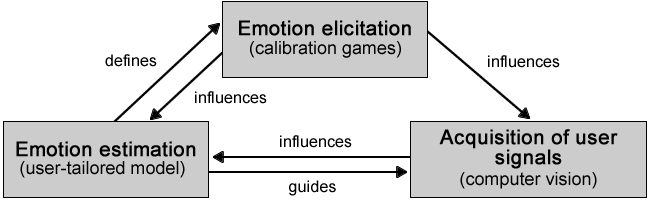
\includegraphics[width=0.8\textwidth]{figures/method-components-dependency.png}
    \caption{tool-ui-face-detector}
    \label{fig:tool-ui-face-detector}
\end{figure}

The output of the face detector is a vector containing 2D points, each one representing a facial landmark. Figure \ref{fig:tool-ui-face-detector} shows a visual representation of the mentioned vector and its points.

\section{Face analyzer}

The face analyzer component uses a frame of the input video and the located face information to extract data regarding facial activity. It contains several different analyzers, each one responsible for extracting specific activity patterns, e.g. eye blink, FACS facial action units, etc. Analyzers are based on the computer vision OpenCV.

Currently the implemented analyzers extract information regarding eye area (for blinking rate), mouth area (for lips/mouth activity), facial center of mass (mean position of all detected landmarks), distance among facial landmarks, face stability (measurement of movement/rotation of the face), and head movement. Figure \ref{fig:tool-ui-face-analyzer} shows the user interface regarding the data provided by the face analyzer.

\begin{figure}[h]
    \centering
    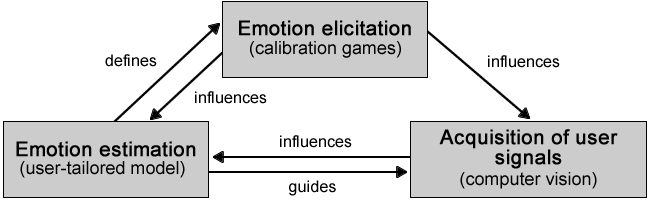
\includegraphics[width=0.8\textwidth]{figures/method-components-dependency.png}
    \caption{fig:tool-ui-face-analyzer}
    \label{fig:tool-ui-face-analyzer}
\end{figure}

\section{Signal estimator}

The signal estimator component uses the frames of the input video and the located face information to estimate user signals, e.g. HR. It contains different estimators, each one responsible for estimating a single signals. Currently two HR estimators are implemented according to the techniques by \textcite{poh2010non} and by \textcite{poh2011advancements}.

Figure \ref{fig:tool-ui-signal-estimator} shows the user interface regarding the data provided by the signal estimator.

\begin{figure}[h]
    \centering
    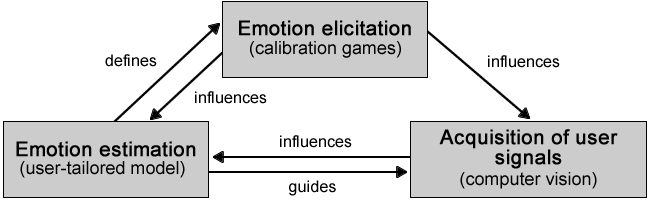
\includegraphics[width=0.8\textwidth]{figures/method-components-dependency.png}
    \caption{fig:tool-ui-signal-estimator}
    \label{fig:tool-ui-signal-estimator}
\end{figure}

\section{Report manager}

The report compoment aggregates the information produced by other components, generating a CSV report file as its output. The report files contains information regarding the video, e.g. time, as well as estimated signals and extracted facial activity. Figure \ref{fig:tool-ui-report-manager} shows part of the content of a report file.

\begin{figure}[h]
    \centering
    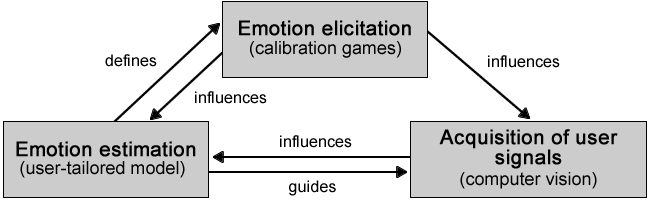
\includegraphics[width=0.8\textwidth]{figures/method-components-dependency.png}
    \caption{fig:tool-ui-report-manager}
    \label{fig:tool-ui-report-manager}
\end{figure}
